%----------------------------------------------------------------------------------------
%	PACKAGES AND DOCUMENT CONFIGURATIONS
%----------------------------------------------------------------------------------------

\documentclass[a4paper,12pt]{article}

\usepackage{amsmath} % Required for some math elements
\usepackage{comment}  % Required for multiline comments
\usepackage{geometry}
\usepackage{subcaption}
\usepackage{graphicx} % Required for the inclusion of images
\usepackage{natbib} % Required to change bibliography style to ABB
\usepackage[linesnumbered,ruled,vlined,algo2e]{algorithm2e} % Required for presenting algorithms
\usepackage{setspace} % This is used in the title page
\usepackage{times}
\usepackage{listings}
\usepackage{color}
\usepackage{enumitem}
\usepackage{dirtree}
\usepackage{caption}

\setlist{nolistsep}
\captionsetup{justification=centering}
\definecolor{anti-flashwhite}{rgb}{0.95, 0.95, 0.96}
\definecolor{dkgreen}{rgb}{0,0.6,0}
\definecolor{gray}{rgb}{0.5,0.5,0.5}
\definecolor{mauve}{rgb}{0.58,0,0.82}
\lstset{frame=single,
  language=Java,
  aboveskip=3mm,
  belowskip=3mm,
  showstringspaces=false,
  columns=flexible,
  basicstyle={\footnotesize\ttfamily},
  numbers=none,
  numberstyle=\tiny\color{gray},
  keywordstyle=\color{blue},
  commentstyle=\color{dkgreen},
  stringstyle=\color{mauve},
  breaklines=true,
  breakatwhitespace=true,
  tabsize=3
}

\newcommand{\newpar}{\smallskip\noindent} %command to create new paragraph with no ident.
\newcommand{\commenter}[3]{$[$\uppercase{#1}#2:#3$]$  \\}
\newcommand{\vitali}[2]{\commenter{vitali}{#1}{#2}}
\newcommand{\maor}[2]{\commenter{maor}{#1}{#2}}
%----------------------------------------------------------------------------------------
%	DOCUMENT INFORMATION
%----------------------------------------------------------------------------------------
\begin{document}

\newgeometry{top=2cm, bottom=2cm, right=2cm, left=2cm}

\begin{center}

\includegraphics{Figures/bgu}\\
{\large Ben-Gurion University of the Negev \\ Faculty of Engineering Science \\ Department of Information Systems Engineering} \\
\vspace*{2mm}
\begin{spacing}{1.5}
\textbf{Final Report} \\
{\LARGE \uppercase{OCCT: One-Class Clustering Tree \\ Implementation for Weka}}
\end{spacing}
\vspace*{2mm}
{\large \textbf{Vitali Sepetnitsky, Maor Tal}} \\
\vspace*{2mm}
\textbf{Instructor:} Dr. Asaf Shabtai \\
\vspace*{2mm}
\textbf{\date{\today}} % Date for the report
\end{center}
%----------------------------------------------------------------------------------------
%	SECTION 1 - Introduction
%----------------------------------------------------------------------------------------
\vspace*{-1.5cm}
\section{Introduction}
\begin{spacing}{1.5}
Data linkage is the task of identifying different entries (i.e., data items) that refer to the same
entity across different data sources \cite{damaging2011}, \cite{kamra2008detecting}. Record linkage refers to the task of joining datasets
that do not share a common identifier (i.e., a foreign key).

\subsection{OCCT}
The two common types of data linkage are:
\begin{itemize}
  \item \emph{one-to-one} data linkage in which the goal is to associate
an entity from one dataset with a single matching entity from the another dataset.
  \item \emph{one-to-many} where the goal is to associate an entity from the first
   dataset to a group of matching entities from the other dataset.
\end{itemize}
\newpar{OCCT} (One-Class Clustering Tree) is a novel data linkage method, presented in \cite{dror2011thesis} and \cite{dror2014occt},
which is capable of performing one-to-many data linkage between entities of same or different
types. The tree is built such that it is easy to transform it into association rules.

One of the major advantages of OCCT compared to other data linkage methods, is using the
one-class approach. This means that it needs only examples of matching pairs in order to learn
and build the model. This feature is important since in many domains it is difficult to obtain
nonmatching examples (e.g. the fraud detection domain).

Building the tree requires deciding which attribute should be selected at each level. There are
four different “splitting criteria” proposed by the authors in \cite{dror2014occt}, along with two pre-pruning process,
to stop expanding branches that does not improve the accuracy of the model.

Once the construction of the tree is completed, a set of probabilistic models are induced for each
of the leafs of the tree.
Each model is deriving the probability of a value of a given attribute from table ($T_{B}$) that
is most likely to be linked with a record from the first table ($T_{A}$).

\subsection{Weka}
Weka (Waikato Environment for Knowledge Analysis) is a suite of machine learning software
which contains a collection of algorithms and visualization tools for data analysis and machine
learning, along with graphical user interfaces for easy access to its functionality. Weka is
free software available under the GNU General Public License.
It is written in Java and developed at the University of Waikato, New Zealand. Weka is also well-suited
for developing new machine learning schemes.

%----------------------------------------------------------------------------------------
%	SECTION 2 - Motivation, Project Goals
%----------------------------------------------------------------------------------------
\section{Motivation}
Dror et al.~\cite{dror2011thesis,dror2014occt} evaluated OCCT as a part of a detection system framework
designed for detecting potential data leakage/misuse. The detection system was
designed to incorporate multiple detectors as plug-ins, where each detector implements a
different detection algorithm, such as OCCT.

The original implementation suffered from many drawbacks, especially it was designed for a
specific domain and did not use any common interfaces which are used in Weka. This made it impossible to
be used by other researchers in order to perform more extensive evaluation and research on OCCT.
In addition evaluating OCCT versus other data linkage algorithms which are already implemented within Weka
was a tedious task.

Our project goal is to implement OCCT, using Weka common API for machine learning
algorithms, and provide basic evaluation of OCCT using our implementation. We intend to add
OCCT as one of the classifiers in Weka UI and make it available to researchers who wishes to further
evaluate OCCT.

%----------------------------------------------------------------------------------------
%	SECTION 3 - Code Structure
%----------------------------------------------------------------------------------------
\section{Code Structure}
The code was carefully designed in order to be flexible for future extensions and also be as readable as possible. Its implementation is based on the J48, which is an open source Java implementation of the C4.5 algorithm in Weka.

\subsection{Packages}
The packages structure of the code can be seen in Figure \vitali{TODO}. This structure allows an easy merge process with the existing Weka source code. The parent packages are {\em src.main.java.weka} which is similar to Weka packages. Then, inside the {\em weka} package, there is {\em classifiers} package which contains different classifiers. Since our implementation was inspired from J48, we placed the main class in file {\em occt.java} inside {\em src.main.java.weka.trees.classifiers}. Other parts of the implementation are located inside {\em trees.occt} package.

The {\em occt} package was divided to three packages: {\em split}, {\em tree} and {\em utils}. The first package, {\em split} contains all the parts of implementation which refer to the splitting criteria. There are several packages inside. We explain some of them below:
\begin{description}
  \item[general] Here we have general classes which helps us to access the spit criterions and pruning methods in a common way.
  \item[iterators] This package contains classes to iterate over the instances in different ways, while calculating the splitting scores.
  \item[models] This package contains an implementation of the four split criteria proposed in \cite{dror2011thesis} and \cite{dror2014occt}.
  \item[pruning] Here we placed all the implementation of the two proposed pruning methods.
\end{description}
The {\em tree} package contains the implementation of the tree structure for representing internal nodes and leafs of the tree which are built during the training phase and queried during the testing phase. Finally, the {\em utils} package contains some general auxiliary classes which are used in the implementation.

\subsection{How It Works?}
Like in J48, the main class is called by the name of the algorithm - OCCT. The training is done via the {\em buildClassifier(Instances)} method which creates the root of the tree of the type {\em OCCTInternalClassifierNode} and calls its local {\em buildClassifier(Instances)} method.

\subsubsection{General}
The algorithm tries to recursively split the dataset contained in each node into subsets. Each internal node, represented by an instance of te {\em OCCTInternalClassifierNode} class, uses an attribute selection method (represented by the {\em OCCTSplitModelSelection} class), which tries to choose the best attribute for split. For this purpose, it evaluates the 'score' for each split (each attribute from $T_A$ defines a split) using an instance of {\em OCCTSingleAttributeSplitModel}.


\subsubsection{Splitting}
The split model can be of instance of one of the four proposed split criteria, e.g. represented by the {\em OCCTMaximumLikelihoodEstimationSplitModel class}. The base class for all the split criteria is {\em OCCTSingleAttributeSplitModel}. This class contains methods for performing basic operations like calculating intersection and union between sets of instances which is required for some of the split criterions. \vitali{TO BE CONTINUED}.

\subsubsection{Leafs}
Each leaf of the tree is represented by the {\em OCCTLeafNodeClass} class and contains the built probabilistic models (which are represented by the {\em ProbModelsHandler} class). Also, as mentioned in \cite{dror2011thesis} and \cite{dror2014occt}, there is no need to save models for all possible attributes of $T_B$. Thus, a feature selection process is executed on the leaf dataset in order to choose the attributes that will be represented by the leafs. This is done by the {\em OCCTFeatureSelector} class which is instantiated for each internal node and extracts the attributes of leafs in case this node has leafs as children.



\clearpage
\subsection{Main structure}
\begin{figure}[!h]
    \centering
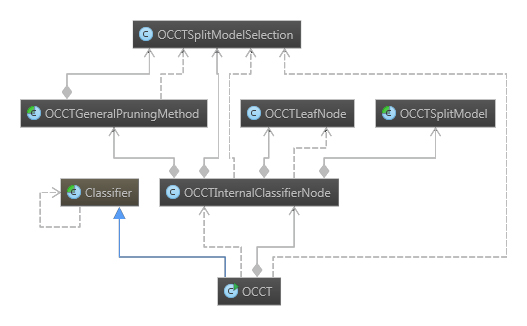
\includegraphics[width=1\textwidth]{Figures/MainStructure}
    \caption{Main OCCT structure}
    \label{fig:mainstr}
\end{figure}

\subsubsection{Splitting structure}
\begin{figure}[!h]
    \centering
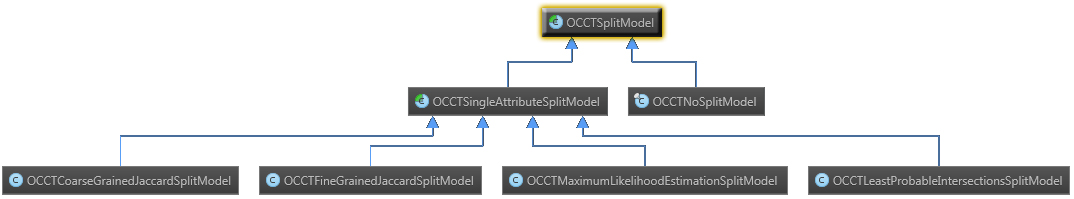
\includegraphics[width=1\textwidth]{Figures/OCCTSplitModelStructure}
    \caption{OCCT Splitting criteria structure}
    \label{fig:splitstr}
\end{figure}
\begin{figure}[!h]
    \centering
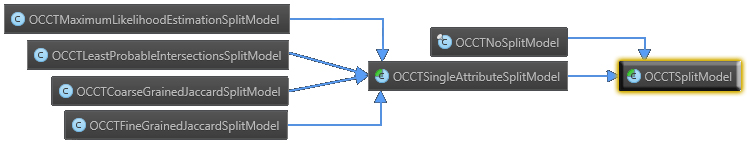
\includegraphics[width=1\textwidth]{Figures/OCCTSplitModelStructure2}
    \caption{OCCT Splitting criteria structure}
    \label{fig:splitstr}
\end{figure}
\clearpage
\subsubsection{Prunning structure}
\begin{figure}[!h]
    \centering
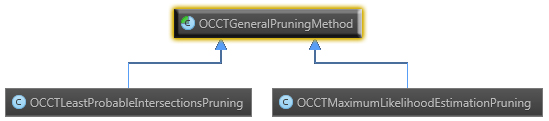
\includegraphics[width=1\textwidth]{Figures/OCCTPruneStructure}
    \caption{OCCT Prunning structure}
    \label{fig:prunestr}
\end{figure}



\clearpage
%----------------------------------------------------------------------------------------
%	SECTION 4 - Deployment
%----------------------------------------------------------------------------------------
\section{Deployment}
We will describe how to install and deploy our implementation of OCCT into a working source code of Weka.
For simplicity we will describe the installation procedure under linux.

\subsection{Dependencies}
Please make sure you have Ant, GIT, Subversion, installed.
if that is not the case, please use the following command:
\begin{lstlisting}[language=bash,frame=none,backgroundcolor=\color{anti-flashwhite}]
  $ sudo apt-get install ant subversion git
\end{lstlisting}

\subsubsection{Obtain Weka source code}
The OCCT code was implemented and evaluated on Weka stable version 3.6.12.
You will now have to checkout that specific branch by using the following svn checkout command:
\begin{lstlisting}[language=bash,frame=none,backgroundcolor=\color{anti-flashwhite}]
  $  svn co https://svn.cms.waikato.ac.nz/svn/weka/tags/stable-3-6-12 Weka-3-6-12
\end{lstlisting}
\newpar
A new directory named '{\em Weka-3-6-12}', will be created once the checkout procedure is done.
The directory structure will be as follows:
\begin{figure}[!h]
\dirtree{%
.1 Weka-3-6-12.
.2 installer.
.3 \ldots{}.
.2 weka.
.3 build.
.3 lib.
.3 resources.
.3 src.
.4 main.
.5 java \begin{minipage}[t]{5cm} \textbf{$\textbf{<}$--- Please go here}\end{minipage}.
.6 weka.
.4 test.
.5 \ldots{}.
.2 wekadocs.
.3 \ldots{}.
.2 wekaexamples.
.3 \ldots{}.
}
    \caption{Weka directory structure}
    \label{fig:wekadir}
\end{figure}

\subsection{Installation}
OCCT code structure was carefully designed for fast deployment into Weka's working source code.
Before we fetch the latest build you first need get into the right path as shown in Fig.~\ref{fig:wekadir}.
\begin{lstlisting}[language=bash,frame=none,backgroundcolor=\color{anti-flashwhite}]
  $ cd Weka-3-6-12/weka/src/main/java
\end{lstlisting}

\subsubsection{Sync with GIT}
Once in {\em Weka-3-6-12/weka/src/main/java} directory you will have to init the GIT repository in-order to obtain the latest source files of our implementation.
Use the following commands to init and sync your local git with our latest build:
\begin{lstlisting}[language=bash,frame=none,backgroundcolor=\color{anti-flashwhite}]
  $ git init
  $ git remote add origin https://github.com/maortal/Weka.OCCT.Classifier.git
  $ git fetch
  $ git checkout -t origin/master
\end{lstlisting}
\newpar
On completion, a new directory named {\em OCCT} and an {\em OCCT.java} file will be added to\\
'{\em Weka-3-6-12/weka/src/main/java/weka/classifiers/trees}' directory.

\subsubsection{Compiling}
Now when the OCCT implementation is merged with Weka's source code, it is time to compile the code.
you need to travel back to '{\em Weka-3-6-12/weka}' directory and run {\em ANT}
\begin{lstlisting}[language=bash,frame=none,backgroundcolor=\color{anti-flashwhite}]
  $ cd ../../../
  $ ant exejar
\end{lstlisting}
Once compilation is complete an executable jar file {\em weka.jar} was generated in a new folder named '{\em dist}'.

%----------------------------------------------------------------------------------------
%	SECTION 5 - GUI Example
%----------------------------------------------------------------------------------------
\clearpage
\section{GUI example}
In this section we will show how to run our OCCT implementation, using Weka's Explorer panel.
\begin{figure}[!h]
  \centering
  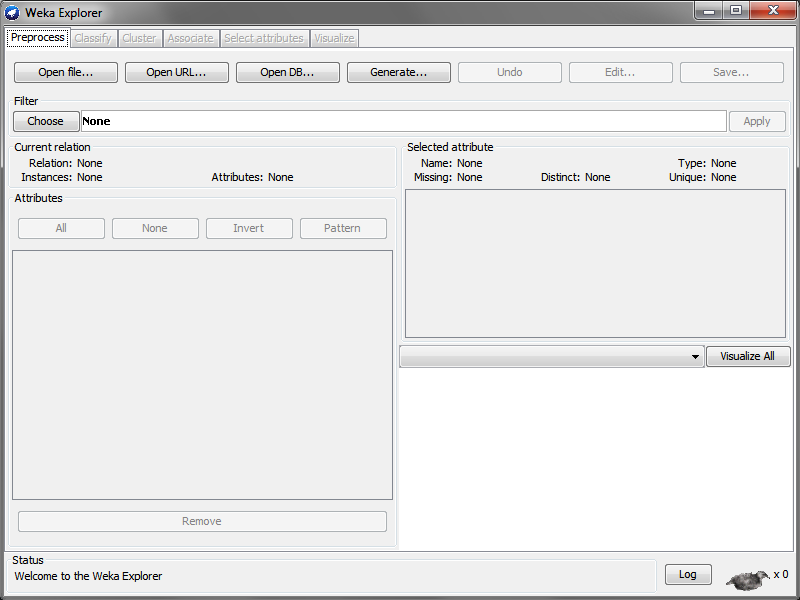
\includegraphics[width=1\textwidth]{Figures/GUI/MainExplorer}\\
  \caption{Explorer Panel}
  \label{fig:wekaexplorer}
\end{figure}
\newpar
In the Explorer panel [Fig~\ref{fig:wekaexplorer}] under {\em Preprocess} tab, click '{\em Open File...}'
and select a database file which is a Cartesian product of two tables $T_{A}$ and $T_{B}$.\\
\clearpage
Under {\em Classify} tab, click on '{\em Choose}' and select {\em OCCT} which is located under {\em tree} classifiers,
as shown in Fig~\ref{fig:occtPre}.
\begin{figure}[!h]
  \centering
  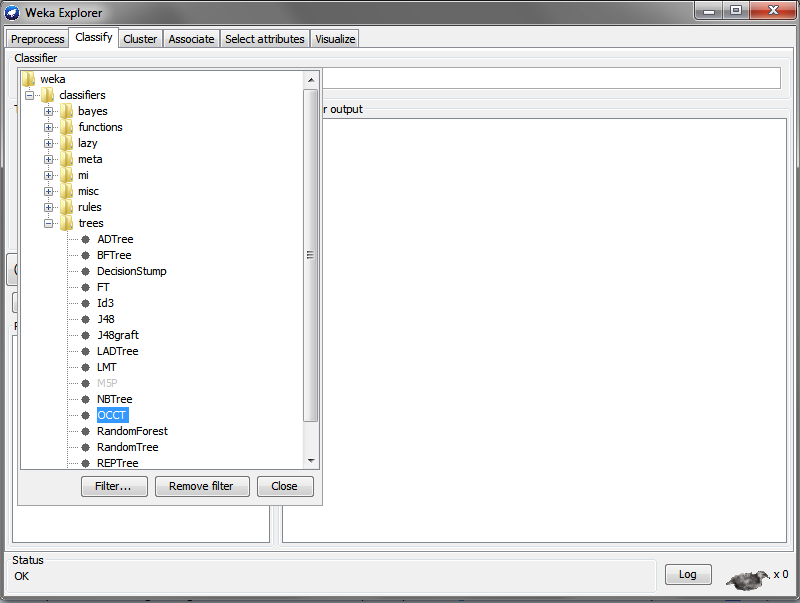
\includegraphics[width=1\textwidth]{Figures/GUI/OCCTPre}\\
  \caption{Classify tab}
  \label{fig:occtPre}
\end{figure}\\


You can now config OCCT's parameters by clicking on the textbox which is located on the right side of the '{\em Choose}' button.
\clearpage
\begin{figure}[!h]
  \centering
  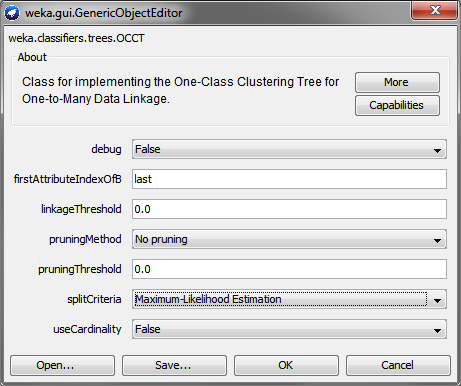
\includegraphics{Figures/GUI/OCCTConfig}\\
  \caption{OCCT parameters config}
  \label{fig:occtconf}
\end{figure}
\begin{itemize}
  \item \textbf{{\em debug}} - boolean flag, whether to print debugging information or not.
  \item \textbf{{\em firstAttribueIndexOfB}} - since OCCT works on Cartesian product of two table, you will need to provide it the
  index in where $T_{B}$ starts from.
  \item \textbf{{\em linkageThreshold}} - In order to determined whether the given records are a match or not, you need to compare the likelihood
  score with a given threshold. If score is greater than the given threshold, it is classified as match.
  \item \textbf{{\em pruningMethod}} - In order to reduce the time complexity of the algorithm, OCCT suggests two prepruning approaches.
  \begin{itemize}
    \item {\em Least-Probable Intersections}
    \item {\em Maximum-Likelihood Estimation}
  \end{itemize}
  \item \textbf{{\em pruningThreshold}} - In order to determined whether to prune a branch or not we need to compare its pruning method score with
  a given threshold.
  \item \textbf{{\em splittingCriteria}} - In order to generate a tree with a small amount of nodes that generalize the data,
  it is crucial to use an effective splitting criterion. OCCT suggests four splitting criteria:
  \begin{itemize}
    \item {\em Coarse-Grained Jaccard}
    \item {\em Fine-Grained Jaccard}
    \item {\em Least-Probable Intersections}
    \item {\em Maximum-Likelihood Estimation}
  \end{itemize}
  \item \textbf{{\em useCardinality}} - boolean flag, whether to use cardinality in the data linkage state or not.
\end{itemize}


%----------------------------------------------------------------------------------------
%	SECTION 6 - Code usage example
%----------------------------------------------------------------------------------------
\clearpage
\section{Code usage example.}
\begin{lstlisting}
	public static void main(String [] argv) throws IOException {
		// load data from arff file
		BufferedReader reader = new BufferedReader(
				new FileReader(new File(argv[0], "database_misuse_example_with_match.arff")));
		Instances data = new Instances(reader);
		reader.close();

        // Train OCCT (don't add any fake class attribute).
		OCCT occt = new OCCT(true);
        // Set debugging mode ON.
		occt.setDebug(true);
        // Set splitting criteria to MLE.
        occt.setSplitCriteria(new SelectedTag(OCCT.SPLIT_MLE, OCCT.TAGS_SPLIT_CRITERIA));
        // Don't use pruning.
        occt.setPruningMethod(new SelectedTag(OCCT.PRUNING_NO_PRUNING, OCCT.TAGS_PRUNING_METHOD));
        // Make the attributes of B be: "City", "CustomerTypeDesc" (+1 since indexes are 1-based)
		occt.setFirstAttributeIndexOfB((data.attribute("City").index() + 1) + "");
        // Define the linkage threshold
		occt.setLinkageThreshold(1.0);
        // Run OCCT and print results
        try {
			occt.buildClassifier(data);
			System.out.println(occt.toString());
			System.out.println("Classification: " +
					occt.classifyInstance(data.firstInstance()));

			//System.out.println(occt.graph()); //print tree in dotfile format
		} catch (Exception e) {
			e.printStackTrace();
			System.exit(-1);
		}
	}
\end{lstlisting}

%----------------------------------------------------------------------------------------
%	SECTION 7 - Evaluation
%----------------------------------------------------------------------------------------
\section{Evaluation}
We evaluated our implementation of OCCT using the same dataset that was used by the authors of OCCT [Table~\ref{ref:datatable}].
A side-by-side comparison of snapshots will be presented in-order to show that our implementation of OCCT algorithm is as intended by the authors.
\begin{table}[h]
\centering
\small
\begin{tabular}{|c|c|c|c|c|c|}\hline
  Request ID & Request Part Of Day & Request Day Of Week & Request Location & Customer City & Customer Type \\\hline
1          & Afternoon           & Friday              & Berlin           & Berlin        & private       \\\hline
2          & Afternoon           & Wednesday           & Hamburg          & Hamburg       & private       \\\hline
3          & Morning             & Wednesday           & Berlin           & Berlin        & business      \\\hline
4          & Morning             & Wednseday           & Berlin           & Berlin        & private       \\\hline
5          & Afternoon           & Saturday            & Berlin           & Berlin        & private       \\\hline
6          & Morning             & Thursday            & Berlin           & Berlin        & private       \\\hline
7          & Afternoon           & Friday              & Berlin           & Berlin        & private       \\\hline
8          & Afternoon           & Saturday            & Berlin           & Berlin        & business      \\\hline
9          & Afternoon           & Saturday            & Berlin           & Berlin        & private       \\\hline
10         & Afternoon           & Friday              & Hamburg          & Hamburg       & business      \\\hline
11         & Afternoon           & Monday              & Hamburg          & Hamburg       & business      \\\hline
12         & Afternoon           & Saturday            & Hamburg          & Hamburg       & private       \\\hline
13         & Afternoon           & Monday              & Berlin           & Berlin        & private       \\\hline
14         & Afternoon           & Monday              & Berlin           & Bonn          & private       \\\hline
15         & Afternoon           & Monday              & Berlin           & Berlin        & private       \\\hline
16         & Morning             & Saturday            & Bonn             & Bonn          & private       \\\hline
17         & Morning             & Saturday            & Hamburg          & Hamburg       & private       \\\hline
18         & Morning             & Saturday            & Hamburg          & Hamburg       & private       \\\hline
19         & Afternoon           & Friday              & Hamburg          & Hamburg       & private       \\\hline
20         & Afternoon           & Friday              & Hamburg          & Bonn          & private       \\\hline
21         & Morning             & Friday              & Hamburg          & Berlin        & private       \\\hline
22         & Morning             & Friday              & Berlin           & Berlin        & business      \\\hline
23         & Morning             & Friday              & Berlin           & Berlin        & private       \\\hline
24         & Afternoon           & Wednseday           & Berlin           & Berlin        & private       \\\hline
25         & Afternoon           & Thursday            & Berlin           & Berlin        & private       \\\hline
26         & Afternoon           & Thursday            & Berlin           & Berlin        & business      \\\hline
27         & Afternoon           & Monday              & Bonn             & Bonn          & business      \\\hline
28         & Afternoon           & Monday              & Bonn             & Hamburg       & private       \\\hline
29         & Afternoon           & Monday              & Bonn             & Berlin        & business      \\\hline
30         & Afternoon           & Wednseday           & Bonn             & Bonn          & business      \\\hline
31         & Afternoon           & Friday              & Bonn             & Bonn          & private       \\\hline

\end{tabular}
\caption{Dataset that was used in our evaluation}
\label{ref:datatable}
\end{table}



\clearpage
\subsection{MLE splitting criteria without pruning}
Presenting the decision model which was induced from the training set, when used MLE splitting criteria without pruning method.

\begin{figure}[!h]
  \centering
  \begin{subfigure}[!h]{1\textwidth}
  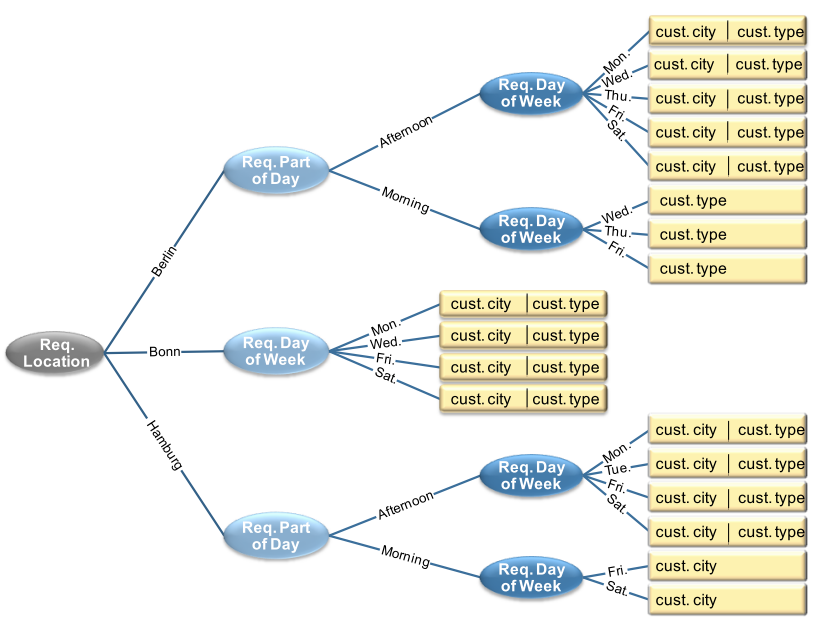
\includegraphics[width=1\textwidth]{Figures/Eval/MaayanMLEnoP}
  \caption{Dror. M \cite{dror2011thesis}, decision model MLE no pruning.}
\end{subfigure}

\begin{subfigure}[!h]{1\textwidth}
  \centering
  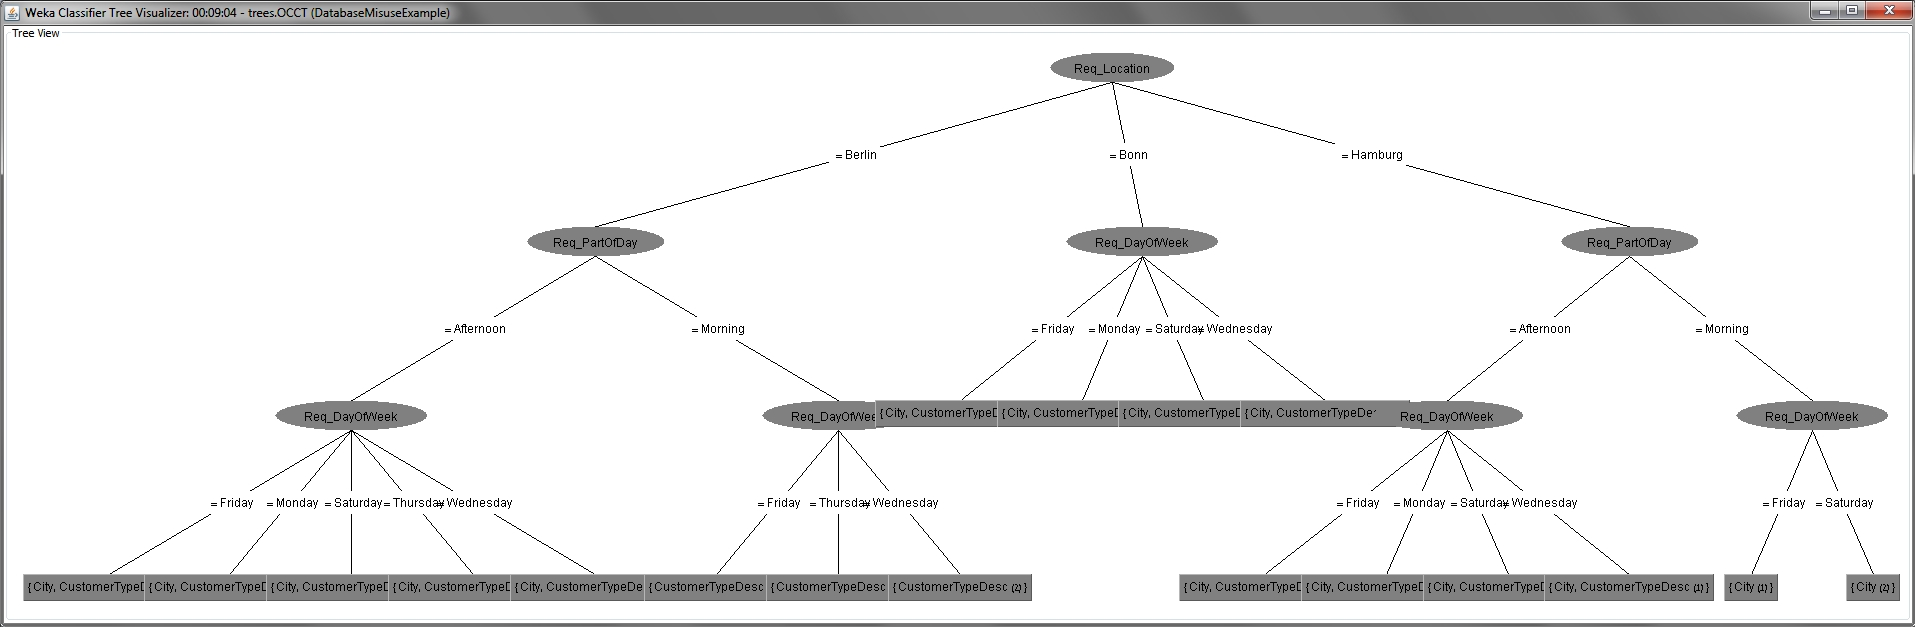
\includegraphics[width=1\textwidth]{Figures/Eval/TreeOut}
  \caption{Our implementation of OCCT, using MLE splitting criteria without pruning.\\ snapshot taken from Weka tree visualizer}
\end{subfigure}
\end{figure}

\subsection{MLE splitting criteria with pruning}
Presenting the decision model which was induced from the training set, when used MLE splitting criteria and appling MLE pruning.

\begin{figure}[!h]
  \centering
  \begin{subfigure}[!h]{1\textwidth}
  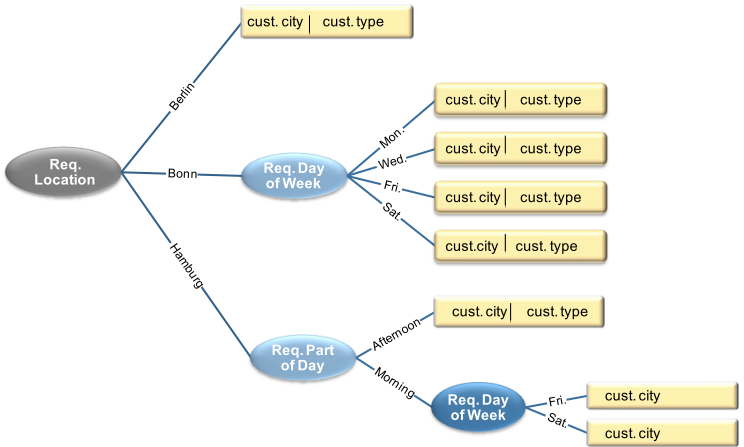
\includegraphics[width=1\textwidth]{Figures/Eval/MaayanMLEwP}
  \caption{Dror. M \cite{dror2011thesis}, decision model MLE with MLE pruning.}
\end{subfigure}

\begin{subfigure}[!h]{1\textwidth}
  \centering
  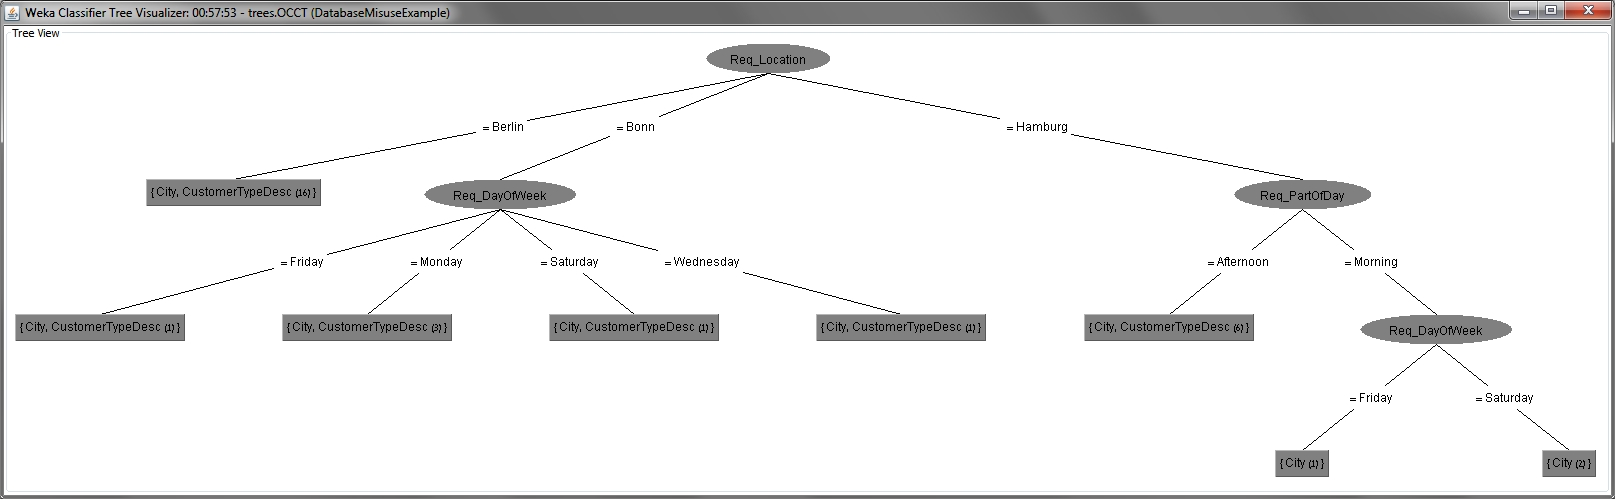
\includegraphics[width=1\textwidth]{Figures/Eval/TreeOutwP}
  \caption{Our implementation of OCCT, using MLE splitting criteria and MLE pruning method.\\ snapshot taken from Weka tree visualizer}
\end{subfigure}
\end{figure}


%----------------------------------------------------------------------------------------
%	SECTION 8 - Future Work
%----------------------------------------------------------------------------------------
\section{Future Work and Extensions}
\begin{comment}
The major drawback of OCCT which has not been overcame in the implementation is too many possible configurations (four splitting criteria and two pruning methods). Thus, a characterization is required in order to decide which splitting criteria and pruning method should be used in each type of domain.
\end{comment}

There is still a lot of work that can be done in order to improve and extend the current implementation and allow it to be ran on more datasets.

First, as noted in \cite{dror2011thesis}, the proposed OCCT algorithm is only capable of handling discrete data. Thus, it cannot analyze attributes that consist of continuous values. In case either $T_A$ or $T_B$ has such attributes, some kind of discretization must be applied in order to make them semi-nominal. This discretization must be done during a preprocess step, before running OCCT. In the current version of the implementation, Weka disables the possibility to ran the algorithm on datasets if they have at least one attribute that is not nominal. This is implemented by using the {\em Capabilities} class of Weka, which ensures that features (e.g. handling certain types of attributes) are enabled explicitly. Our suggestion is to implement this missing functionality and allow OCCT to handle both continuous and discrete attributes. For example, handling continuous attributes can be implemented in the same way of C4.5, which creates a threshold and then splits the instances into those whose attribute value is above the threshold and those that are less than or equal to it.

Other problem with the current implementation refers to the input format of the algorithm; currently, OCCT is referred as a classification algorithm, which means that it is located in the Classify tab of Weka and uses the common GUI of a classifier. However, OCCT purpose is solving data linkage problems. The uniqueness of these problems is receiving two datasets as an input and also irrelevant class attribute of the dataset. This type of input does not exist in the Classify tab of the GUI chooser of Weka. Currently, in order to overcome that problem of receiving two datasets as an input, we added an input index, which defines the first column of $T_B$ in the input. Since the input of the algorithm is a training set of only matching instances $T_AB \subseteq T_A \times T_B$, it is sufficient for now. However, Weka has an option of adding extra tabs in the Explorer in order to add new functionality without the hassle of having to dig into the code of the Explorer. We suggest to add a new tab for data linkage algorithms. This tab should be similar to the Classify tab, but it will allow the user to choose two different datasets for $T_A$ and $T_B$.




%----------------------------------------------------------------------------------------
\bibliographystyle{unsrt}
\bibliography{refFile}
\restoregeometry
\end{spacing}

\end{document}
